% Modified based on Xiaoming Sun's template
\documentclass{article}
\usepackage{amsmath,amsfonts,amsthm,amssymb}
\usepackage{setspace}
\usepackage{fancyhdr}
\usepackage{lastpage}
\usepackage{extramarks}
\usepackage{chngpage}
\usepackage{soul,color}
\usepackage{graphicx,float,wrapfig}
\usepackage{enumitem}
\usepackage{array} 
\usepackage{hyperref}
\usepackage{float}
\usepackage{fontspec}
\setmonofont{Consolas}
\usepackage{listings}
\usepackage{xcolor}
\lstset{
  language = python, numbers=left, 
         numberstyle=\tiny,keywordstyle=\color{blue!70},
         commentstyle=\color{red!50!green!50!blue!50},frame=shadowbox,
         rulesepcolor=\color{red!20!green!20!blue!20},basicstyle=\ttfamily
}
\renewcommand{\d}{\mathrm{d}}
\newcommand{\Class}{Pattern Recognition and Machine Learning}

% Homework Specific Information. Change it to your own
\newcommand{\Title}{Homework 2}

% In case you need to adjust margins:
\topmargin=-0.45in      %
\evensidemargin=0in     %
\oddsidemargin=0in      %
\textwidth=6.5in        %
\textheight=9.0in       %
\headsep=0.25in         %

% Setup the header and footer
\pagestyle{fancy}                                                       %
\chead{\Title}  %
\rhead{\firstxmark}                                                     %
\lfoot{\lastxmark}                                                      %
\cfoot{}                                                                %
\rfoot{Page\ \thepage\ of\ \protect\pageref{LastPage}}                          %
\renewcommand\headrulewidth{0.4pt}                                      %
\renewcommand\footrulewidth{0.4pt}                                      %

%%%%%%%%%%%%%%%%%%%%%%%%%%%%%%%%%%%%%%%%%%%%%%%%%%%%%%%%%%%%%
% Some tools
\newcommand{\enterProblemHeader}[1]{\nobreak\extramarks{#1}{#1 continued on next page\ldots}\nobreak%
                                    \nobreak\extramarks{#1 (continued)}{#1 continued on next page\ldots}\nobreak}%
\newcommand{\exitProblemHeader}[1]{\nobreak\extramarks{#1 (continued)}{#1 continued on next page\ldots}\nobreak%
                                   \nobreak\extramarks{#1}{}\nobreak}%

\newcommand{\homeworkProblemName}{}%
\newcounter{homeworkProblemCounter}%
\newenvironment{homeworkProblem}[1][Problem \arabic{homeworkProblemCounter}]%
  {\stepcounter{homeworkProblemCounter}%
   \renewcommand{\homeworkProblemName}{#1}%
   \section*{\homeworkProblemName}%
   \enterProblemHeader{\homeworkProblemName}}%
  {\exitProblemHeader{\homeworkProblemName}}%

\newcommand{\homeworkSectionName}{}%
\newlength{\homeworkSectionLabelLength}{}%
\newenvironment{homeworkSection}[1]%
  {% We put this space here to make sure we're not connected to the above.

   \renewcommand{\homeworkSectionName}{#1}%
   \settowidth{\homeworkSectionLabelLength}{\homeworkSectionName}%
   \addtolength{\homeworkSectionLabelLength}{0.25in}%
   \changetext{}{-\homeworkSectionLabelLength}{}{}{}%
   \subsection*{\homeworkSectionName}%
   \enterProblemHeader{\homeworkProblemName\ [\homeworkSectionName]}}%
  {\enterProblemHeader{\homeworkProblemName}%

   % We put the blank space above in order to make sure this margin
   % change doesn't happen too soon.
   \changetext{}{+\homeworkSectionLabelLength}{}{}{}}%

\newcommand{\Answer}{\ \\\textbf{Answer:} }
\newcommand{\Acknowledgement}[1]{\ \\{\bf Acknowledgement:} #1}

%%%%%%%%%%%%%%%%%%%%%%%%%%%%%%%%%%%%%%%%%%%%%%%%%%%%%%%%%%%%%


%%%%%%%%%%%%%%%%%%%%%%%%%%%%%%%%%%%%%%%%%%%%%%%%%%%%%%%%%%%%%
% Make title
\title{\textmd{\bf \Class: \Title}}
  \date{\textbf{\today}}
\author{\textbf{Qingru Hu \quad 2020012996}}
%%%%%%%%%%%%%%%%%%%%%%%%%%%%%%%%%%%%%%%%%%%%%%%%%%%%%%%%%%%%%

\begin{document}
\begin{spacing}{1.1}
\maketitle \thispagestyle{empty}

%%%%%%%%%%%%%%%%%%%%%%%%%%%%%%%%%%%%%%%%%%%%%%%%%%%%%%%%%%%%%
% Begin edit from here

\begin{homeworkProblem}
\subsection*{Task1}
\subsubsection*{1.}
Take the object function in Equation(2) into three parts:
\begin{align*}
  f_1 &= \frac{1}{l} \text{Tr}((Y-JKW)^{T}(Y-JKW)) \\
  f_2 &= \gamma_A \text{Tr}(W^T K W) \\
  f_3 &= \frac{\gamma_I}{(u+l)^2}\text{Tr}(W^TKLKW)
\end{align*}
Take the derivative of $f_1$:
\begin{align*}
  \d f_1 &= \frac{1}{l} \text{Tr} (\d (Y-JKW)^{T} (Y-JKW) + (Y-JKW)^{T} \d (Y-JKW)) \\
  &= \frac{2}{l} \text{Tr}((Y-JKW)^{T} \d (Y-JKW)) \\
  &= \frac{2}{l} \text{Tr}((Y-JKW)^{T} (-JK) \d W) \\
  \frac{\d f_1}{\d W} &= -\frac{2}{l} (JK)^{T} (Y-JKW)
\end{align*}
Take the derivative of $f_2$:
\begin{align*}
  \d f_2 &= \gamma_A \text{Tr} (\d W^T K W + W^T K \d W) \\
  &= 2 \gamma_A \text{Tr} (W^T K \d W) \\
  \frac{\d f_2}{\d W} &= 2 \gamma_A K W
\end{align*}
Take the derivative of $f_3$:
\begin{align*}
  \d f_3 &= \frac{\gamma_I}{(u+l)^2}\text{Tr}((\d W^T)KLKW + W^TKLK\d W) \\
  &= \frac{2\gamma_I}{(u+l)^2} \text{Tr}(W^TKLK\d W) \\
  \frac{\d f_3}{\d W} &= \frac{2\gamma_I}{(u+l)^2} KLK W
\end{align*}

The solution for the optimization should satisfy:
\begin{align*}
  \frac{\d f_1}{\d W} + \frac{\d f_2}{\d W} + \frac{\d f_3}{\d W} &= 0 \\
  -\frac{2}{l} (JK)^{T} (Y-JKW) + 2 \gamma_A K W + \frac{2\gamma_I}{(u+l)^2} KLK W &= 0 \\
  ((JK)^{T}JK + \gamma_A l K + \frac{\gamma_I l}{(u+l)^2} KLK)W &= (JK)^{T} Y \\
  \because K^T = K, J^T = J, \text{multiply $K^{-1}$ on both sides to the right} \\
  (JJK + \gamma_A l I + \frac{\gamma_I l}{(u+l)^2} LK)W &= JY \\
  \because JY = Y \\
  W^* = (JJK + \gamma_A l I + \frac{\gamma_I l}{(u+l)^2} LK)^{-1}Y
\end{align*}
From the definition of $J$, we can also have $JJ=J$. Therefore, 
the best solution is:
\begin{align*}
  W^* = (JK + \gamma_A l I + \frac{\gamma_I l}{(u+l)^2} LK)^{-1}Y
\end{align*}

\subsubsection*{2.}
\begin{lstlisting}
  # define Y
  l = len(X_l)
  u = len(X_u)
  X = np.concatenate([X_l, X_u])
  self.X = X
  Y_u = np.zeros([u, Y_l.shape[1]])
  Y = np.concatenate([Y_l, Y_u])

  self.W = np.linalg.inv(J.dot(K) + self.gamma_A*l*np.identity(l+u) 
            + (self.gamma_I*l)/(u+l)**2*L.dot(K)).dot(Y)
\end{lstlisting}

\subsection*{Task2}
The mean of the accuracy of LapRLS is better than that of RLS in two datasets. The std of the two methods are almost the same.
\begin{table}[htbp]
  \centering
  \begin{tabular}{|c|cc|cc|}
  \hline
         & \multicolumn{2}{c|}{digits}         & \multicolumn{2}{c|}{usps}           \\ \hline
         & \multicolumn{1}{c|}{mean}  & std    & \multicolumn{1}{c|}{mean}  & std    \\ \hline
  RLS    & \multicolumn{1}{c|}{0.826} & 0.0378 & \multicolumn{1}{c|}{0.748} & 0.0089 \\ \hline
  LapRLS & \multicolumn{1}{c|}{0.861} & 0.0230 & \multicolumn{1}{c|}{0.893} & 0.0096 \\ \hline
  \end{tabular}
  \end{table}

\subsection*{Task3}
\subsubsection*{1.}
\begin{lstlisting}
from sklearn.decomposition import PCA
from sklearn.discriminant_analysis import LinearDiscriminantAnalysis as LDA
from sklearn.manifold import MDS
from sklearn.manifold import Isomap
from sklearn.manifold import LocallyLinearEmbedding as LLE
from sklearn.manifold import TSNE

methods = {
  'PCA': PCA(n_components=2),
  'LDA':LDA(),
  'MDS':MDS(n_components=2),
  'Isomap':Isomap(n_components=2),
  'LLE':LLE(n_components=2),
  't-SNE':TSNE(n_components=2)
}
\end{lstlisting}

\subsubsection*{2.}
Use the digits dataset for visualization. Visualization results are shown in Fig.1 and Fig.2.

\begin{figure}[htbp]
  \centering
  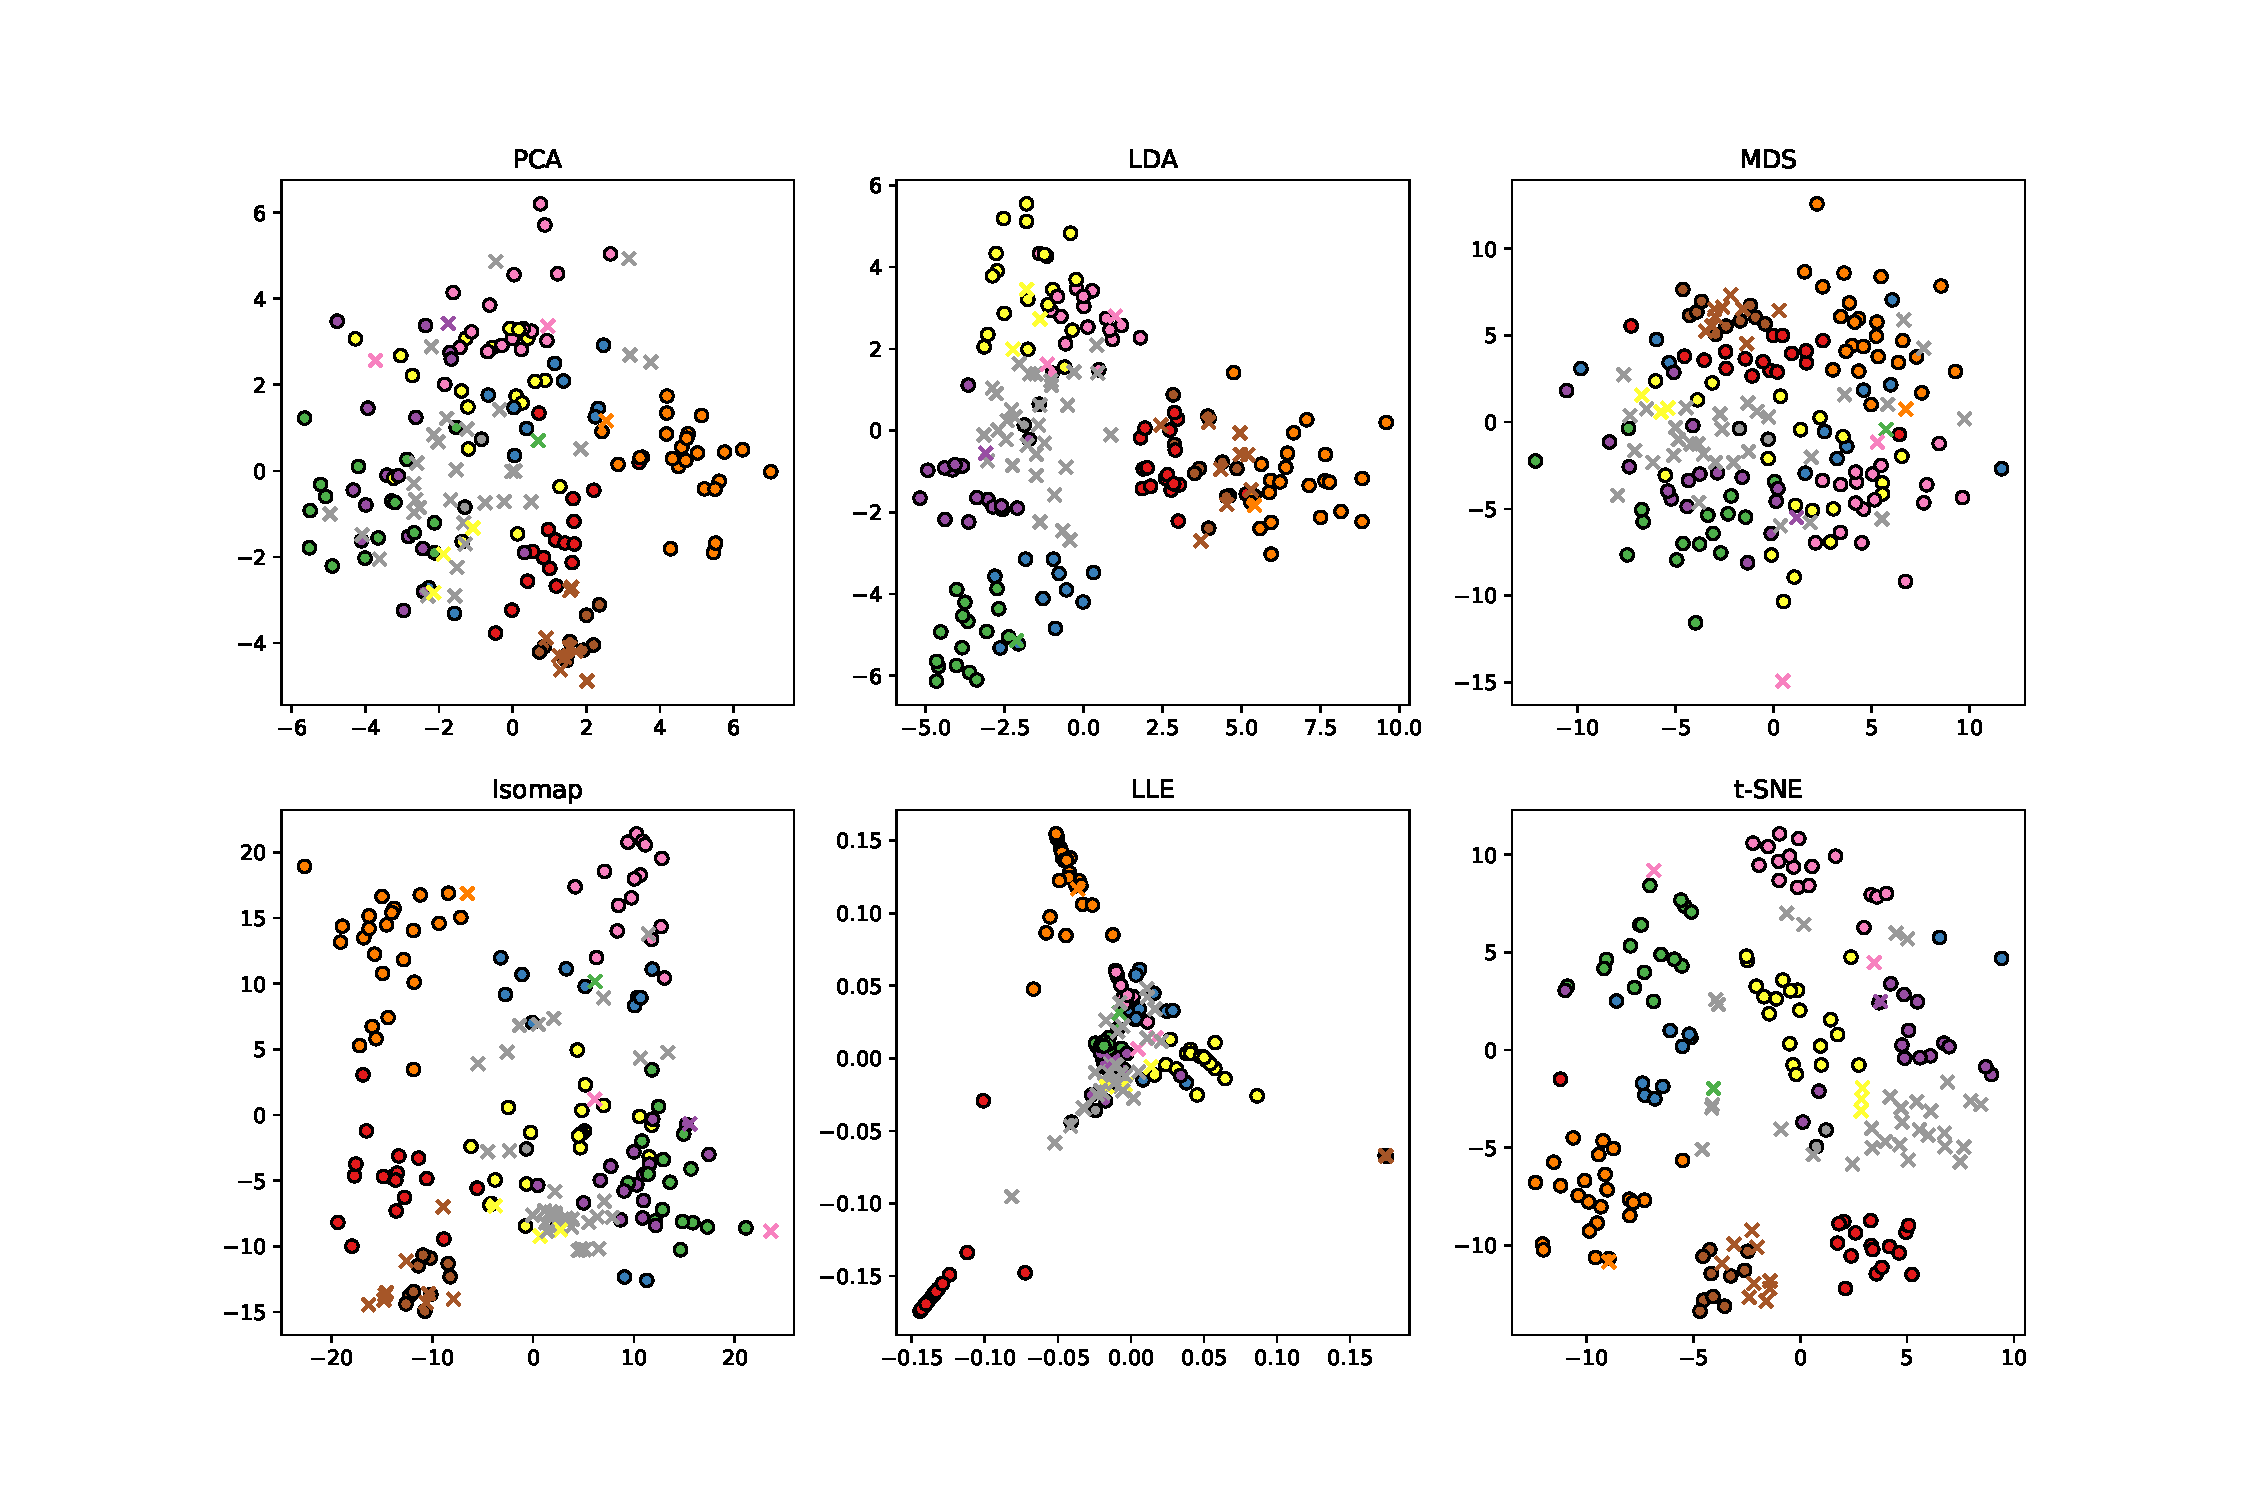
\includegraphics[width=16cm]{rls.pdf}
  \caption{The visualization for RLS}
\end{figure}

\begin{figure}[htbp]
  \centering
  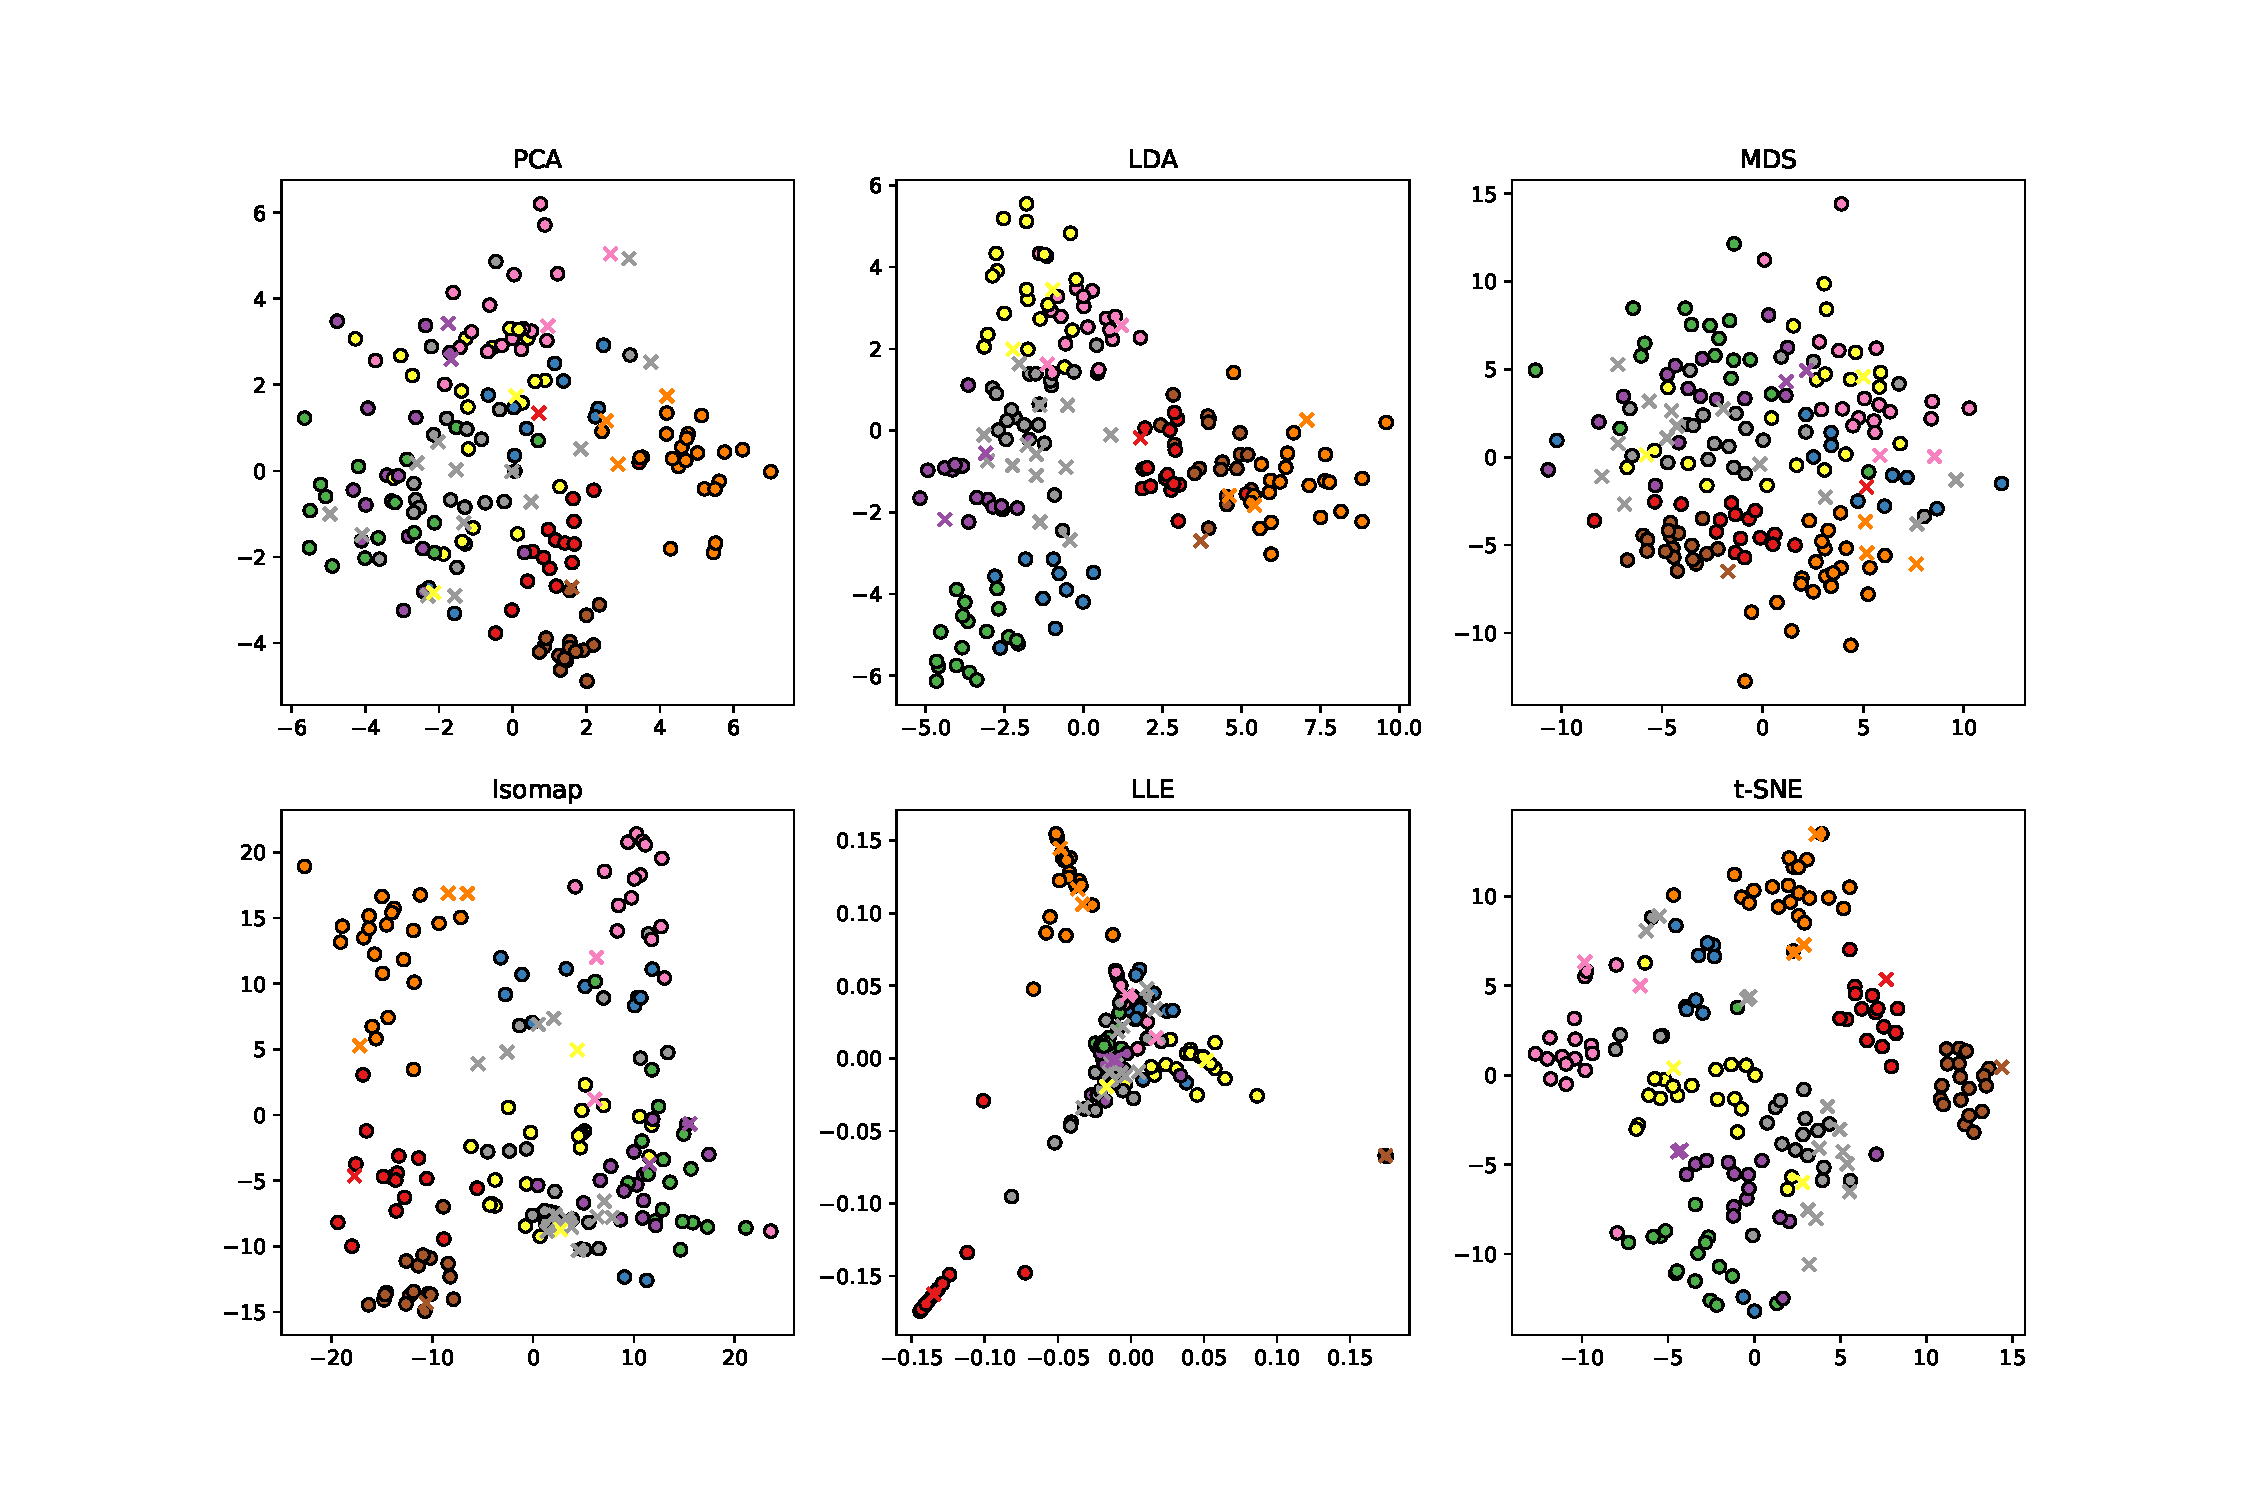
\includegraphics[width=16cm]{laprls.pdf}
  \caption{The visualization for LapRLS}
\end{figure}

\end{homeworkProblem}


% \newpage
% \Acknowledgement{Thank Siying Yang 2020012981 for
% the discussion about Problem 2.3 and Problem 3.}

% End edit to here
%%%%%%%%%%%%%%%%%%%%%%%%%%%%%%%%%%%%%%%%%%%%%%%%%%%%%%%%%%%%%

\end{spacing}
\end{document}

%%%%%%%%%%%%%%%%%%%%%%%%%%%%%%%%%%%%%%%%%%%%%%%%%%%%%%%%%%%%%
